\documentclass[11pt,t]{beamer}

\graphicspath{{Images/}{./}}
\usepackage{booktabs}
\usetheme{Madrid}

\usefonttheme{default} % Typeset using the default sans serif font

\usepackage{palatino} % Use the Palatino font for serif text

\usepackage[default]{opensans} % Use the Open Sans font for sans serif text

\useinnertheme{circles}

\newcommand{\light}[1]{\textcolor{gray}{#1}}
\usepackage{xcolor}

\title[DSA Scale Uncertainty]{Addressing Scale Uncertainty in Gene and Microbe Set Enrichment Analysis}

\author[Kyle McGovern]{Kyle McGovern}

\institute[Penn State]{The Pennsylvania State University \\ \smallskip \textit{kvm6065@psu.edu}} 

\date[\today]{GLBIO 2024 \\ \today}

%----------------------------------------------------------------------------------------

\begin{document}

%----------------------------------------------------------------------------------------
%	TITLE SLIDE
%----------------------------------------------------------------------------------------

\begin{frame}
	\titlepage % Output the title slide, automatically created using the text entered in the PRESENTATION INFORMATION block above
\end{frame}

\begin{frame}
    \frametitle{Review of Key Concepts}

    Consider as an example an 16S rRNA-seq experiment measuring \(D\) taxa in the colons of \(N\) patients:
    \begin{align*}
      \underbrace{W_{dn}}_{\substack{\text{Absolute Abundance} \\ \text{Taxa d, Patient n} \\ \text{\textcolor{red}{(Unmeasured)}}}} = \underbrace{W^\parallel_{dn}}_{\substack{\text{Composition} \\ \text{Taxa d, Patient n} \\ \text{\textcolor{green}{(Measured)}}}} \times \underbrace{W^\perp_n}_{\substack{\text{Scale} \\ \text{(e.g., total \# of microbes in} \\ \text{patient n's colon)} \\ \text{\textcolor{red}{(Unmeasured)}}}}
    \end{align*}

    \pause

    Further consider as an example estimation of the LFC (Log Fold Change) of taxa \(d\) in patients with and without Ulcerative Colitis:
    \begin{align*}
        \underbrace{\theta_d}_{\text{LFC in Absolute Abundance}} &= \underbrace{\theta^{\parallel}_d}_{\text{LFC in Composition}}+\underbrace{\theta^\perp}_{\text{LFC in Scale}}. \nonumber
    \end{align*}

\end{frame}

\begin{frame}
  \frametitle{Review of Key Concepts}

    Methods like ALDEx2, DESeq2, Limma, etc. estimate LFCs using sequence count data \(Y\):
    \begin{align*}
    f(Y) &= \hat{\theta}_d \\
    &= \underbrace{\hat{\theta}^\parallel_d}_{\substack{\text{Estimated LFC in the} \\ \text{\textcolor{green}{measured} composition}}} + \underbrace{\hat{\theta}^\perp}_{\substack{\text{Estimated LFC in the} \\ \text{\textcolor{red}{unmeasured} scale}}}.
    \end{align*}

    \pause

    Estimates \(\hat{\theta}^\perp\) come from normalization, for example:
    \begin{itemize}
      \item Total Sum Scaling (TSS): \(\hat{\theta}^\perp=0\)
      \pause
      \item Centered Log Ratio (CLR): \(\hat{\theta}^\perp=-\text{mean}(\hat{\theta}^\parallel)\)
    \end{itemize}
\end{frame}

\begin{frame}
  \frametitle{Differential Set Analysis (DSA)}

  \begin{columns}
    \begin{column}{0.45\textwidth}
      \begin{center}
        Rather than estimating \textbf{LFCs} of \textbf{single} genes/taxa

        \vspace{50px}
        \includegraphics[scale=0.23]{/home/hh/data/output/one_gene.png}
      \end{center}
    \end{column}
    \vrule{}
    \begin{column}{0.55\textwidth}  
      \begin{center}
        What if we are interested in a \textbf{set} of genes in a pathway?
       \includegraphics[scale=0.23]{/home/hh/data/output/apop_sub.png}
     \end{center}
  \end{column}
  \end{columns}

  \begin{center}
    \textbf{Differential Set Analysis (DSA) is used to estimate enrichment or depletion of a gene/taxa set}
  \end{center}
\end{frame}
  
\begin{frame}
  \frametitle{Key Points of this Talk}

  \begin{enumerate}
  \item Errors in scale assumptions (i.e., estimates \(\hat{\theta}^\perp\), \(\hat{W}^\perp\)) inflate false positive rates in DSA
    \pause
  \item Errors in DSA estimates are a \textbf{non-linear} function of scale errors
    \pause
  \item We have developed three solutions to these errors:
    \begin{enumerate}
      \item LFC Sensitivity Analysis
      \item LFC Sensitivity Testing
      \item Compositional Weighting Methods
    \end{enumerate}
  \end{enumerate}
\end{frame}

\begin{frame}
  \frametitle{Three Methods for DSA}

  In this presentation 3 common DSA methods will be considered
  \begin{enumerate}
    \item \textbf{Gene Set Enrichment Analysis (GSEA) with Gene Label permutations}
    \item Gene Set Enrichment Analysis (GSEA) with Sample Label permutations
    \item CAMERA
  \end{enumerate}
\end{frame}

\begin{frame}
  \frametitle{GSEA with Gene Label Permutations}

  The GSEA Algorithm Step-by-Step
  \begin{enumerate}
  \item Pick a set of genes \(S\) (e.g., the apoptosis signaling pathway):
    \begin{align*}
      S = \{\text{ASK1, CHOP, TRAF2}\}
    \end{align*}
    \pause
  \item Estimate LFCs \(\hat{\theta}=f(Y)\) (i.e., with DESeq2, ALDEx2, limma)
    \pause
    \item Order the LFCs from largest to smallest
    \begin{figure}
      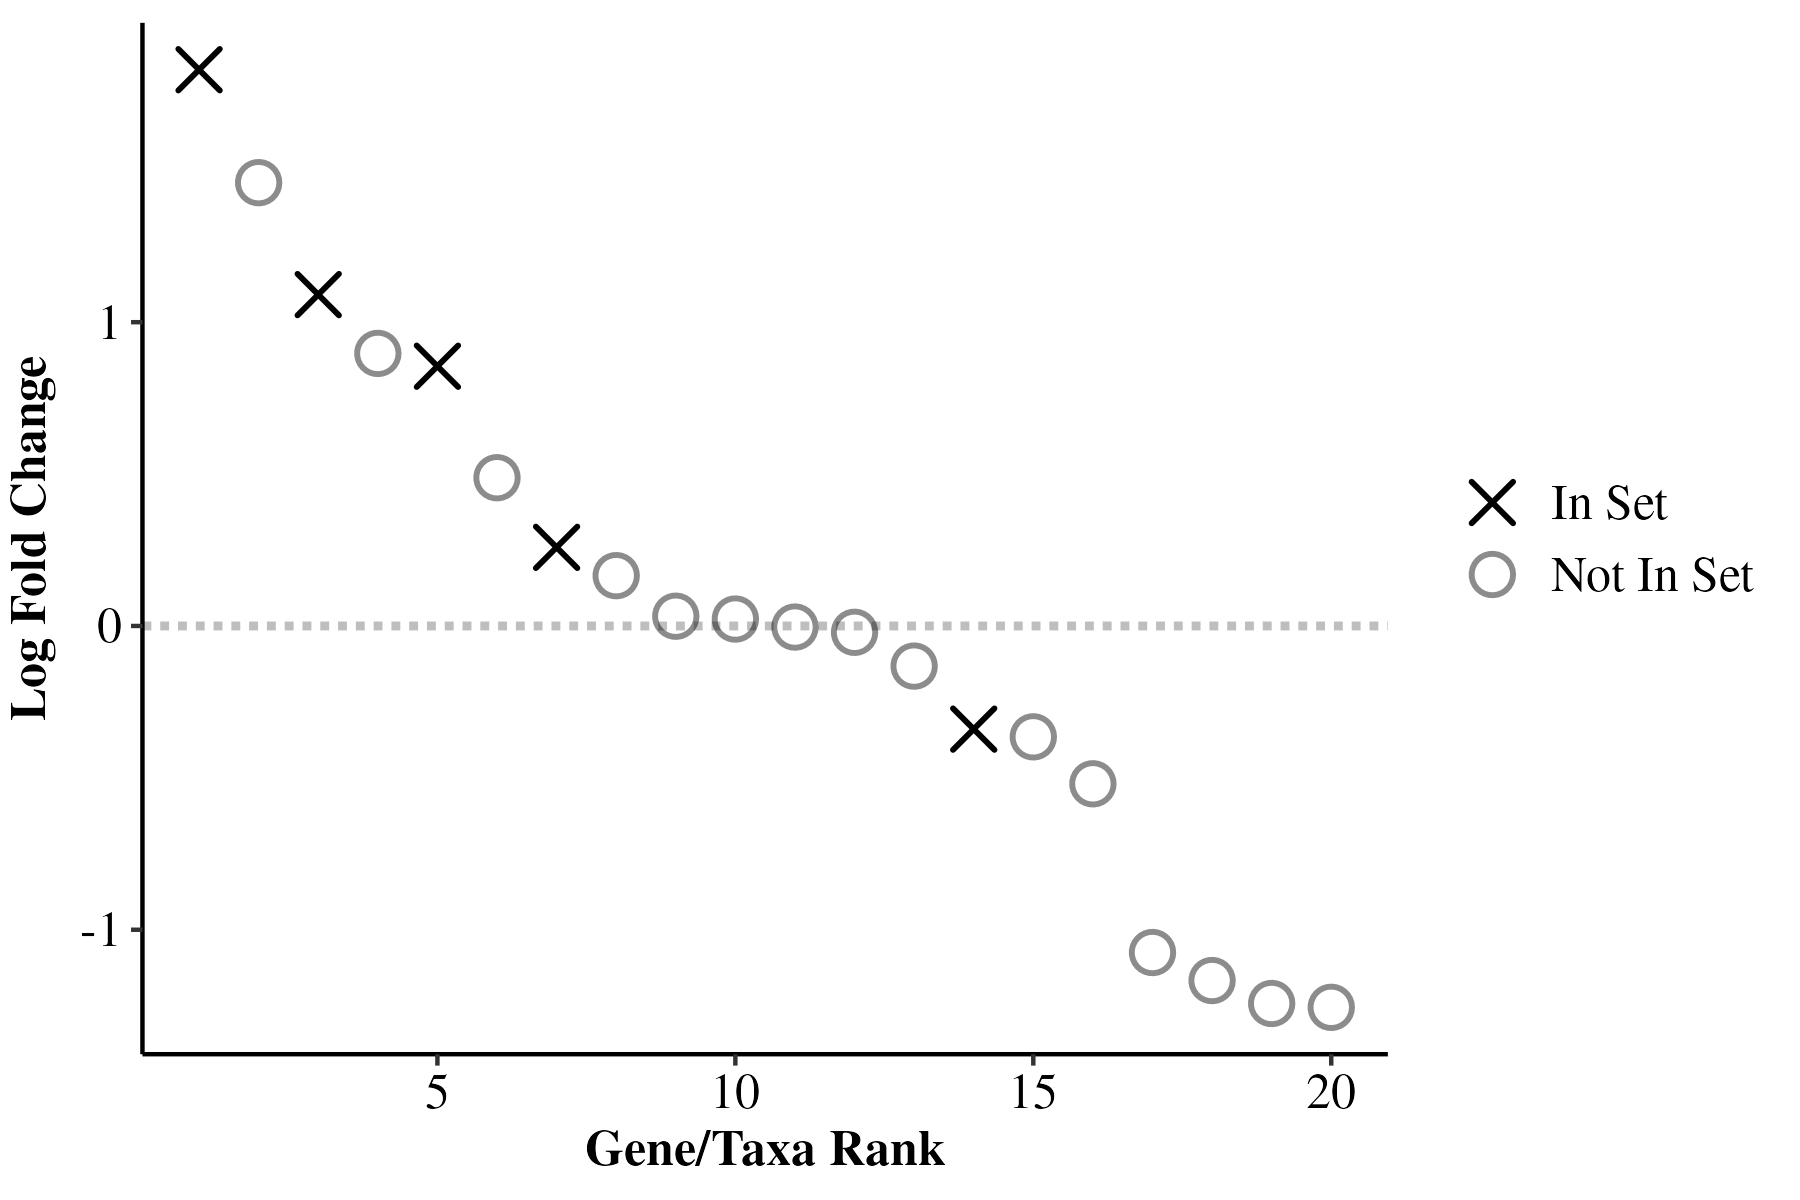
\includegraphics[scale=0.4]{/home/hh/data/output/lfcs_1.png}
      \centering
    \end{figure}
  \end{enumerate}
\end{frame}


\begin{frame}
   \frametitle{GSEA with Gene Label Permutations}

  The GSEA Algorithm Step-by-Step
  \begin{enumerate}
    \setcounter{enumi}{2}
    \item Calculate a running sum \textbf{weighted} by the LFC
    \item Calculate an enrichment score (max distance from \(0\) of \textbf{weighted} running sum)
    \begin{columns}
        \begin{column}{0.5\textwidth}
        \begin{center}
            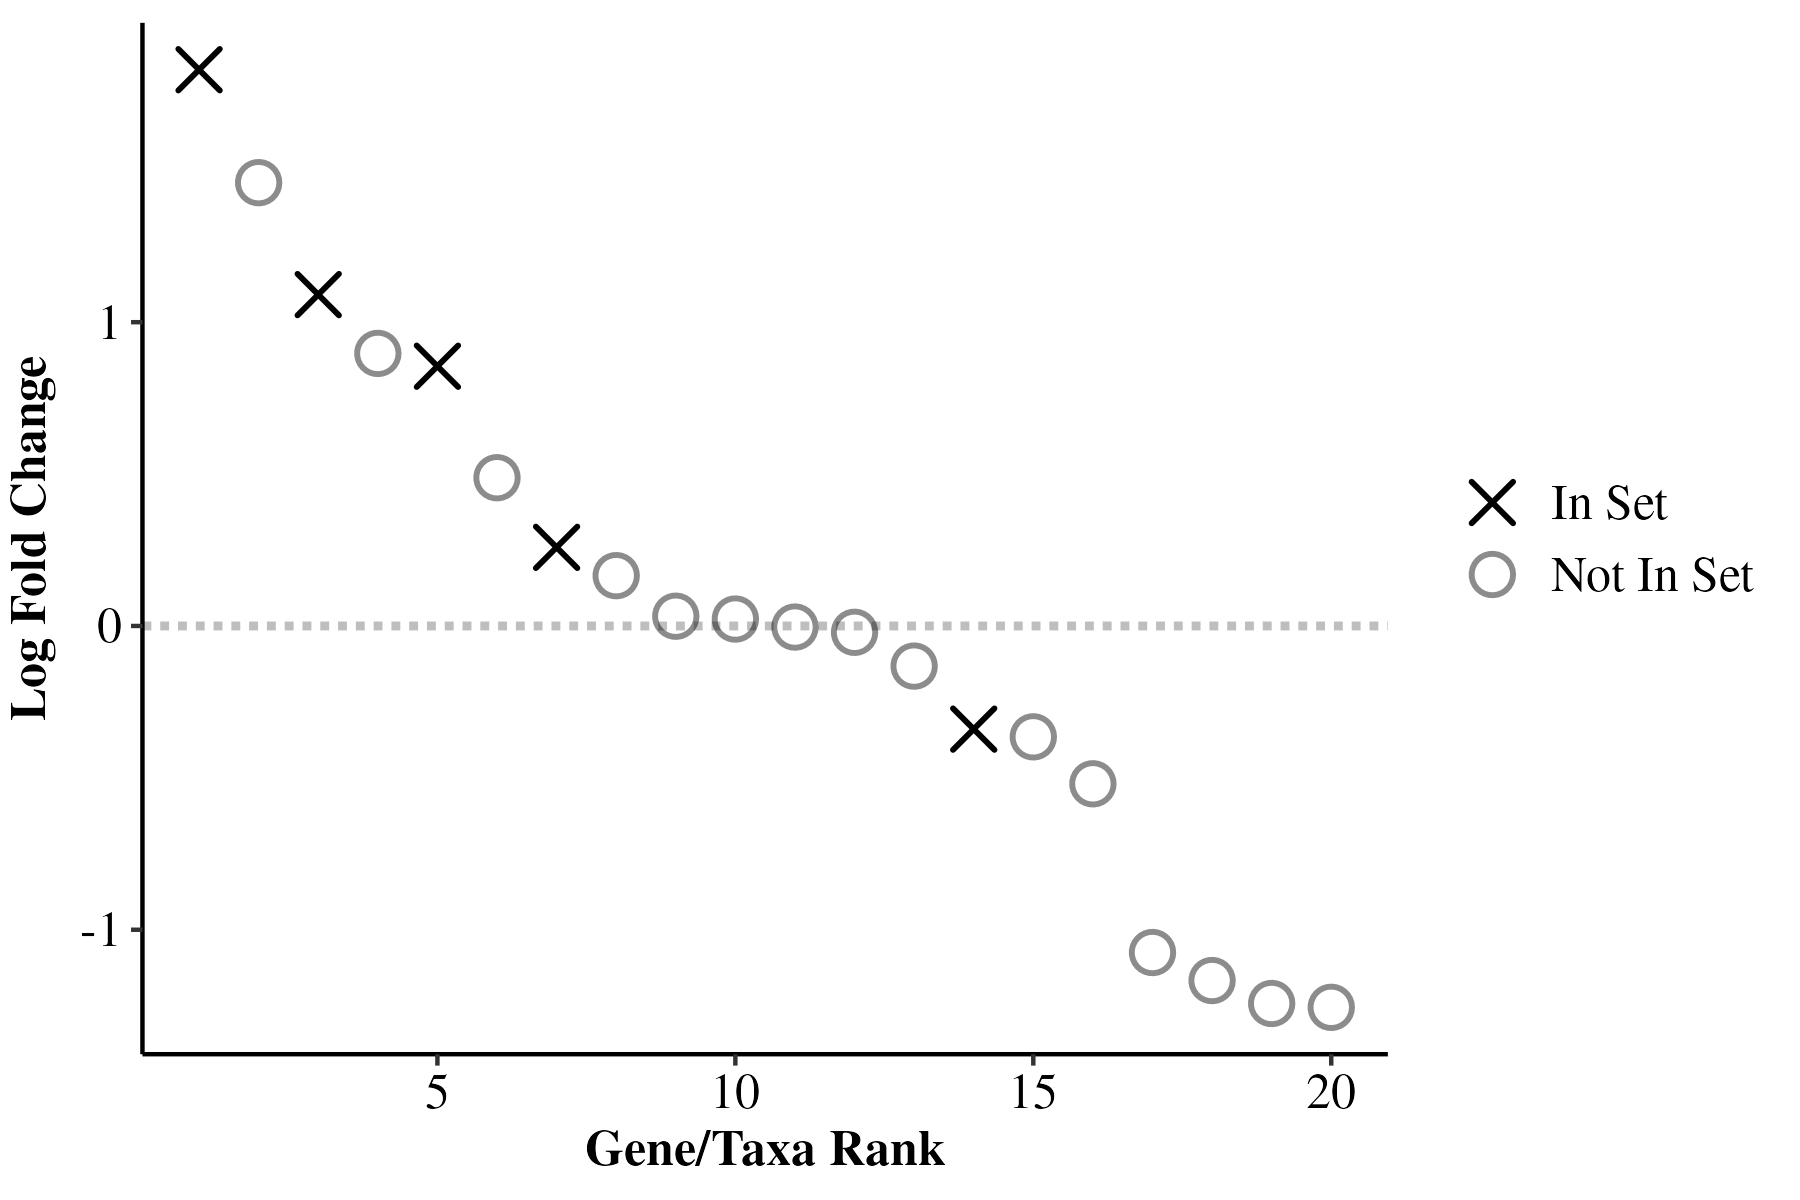
\includegraphics[scale=0.4]{/home/hh/data/output/lfcs_1.png}
        \end{center}
        \end{column}
        \begin{column}{0.5\textwidth}  %%<--- here
        \begin{center}
        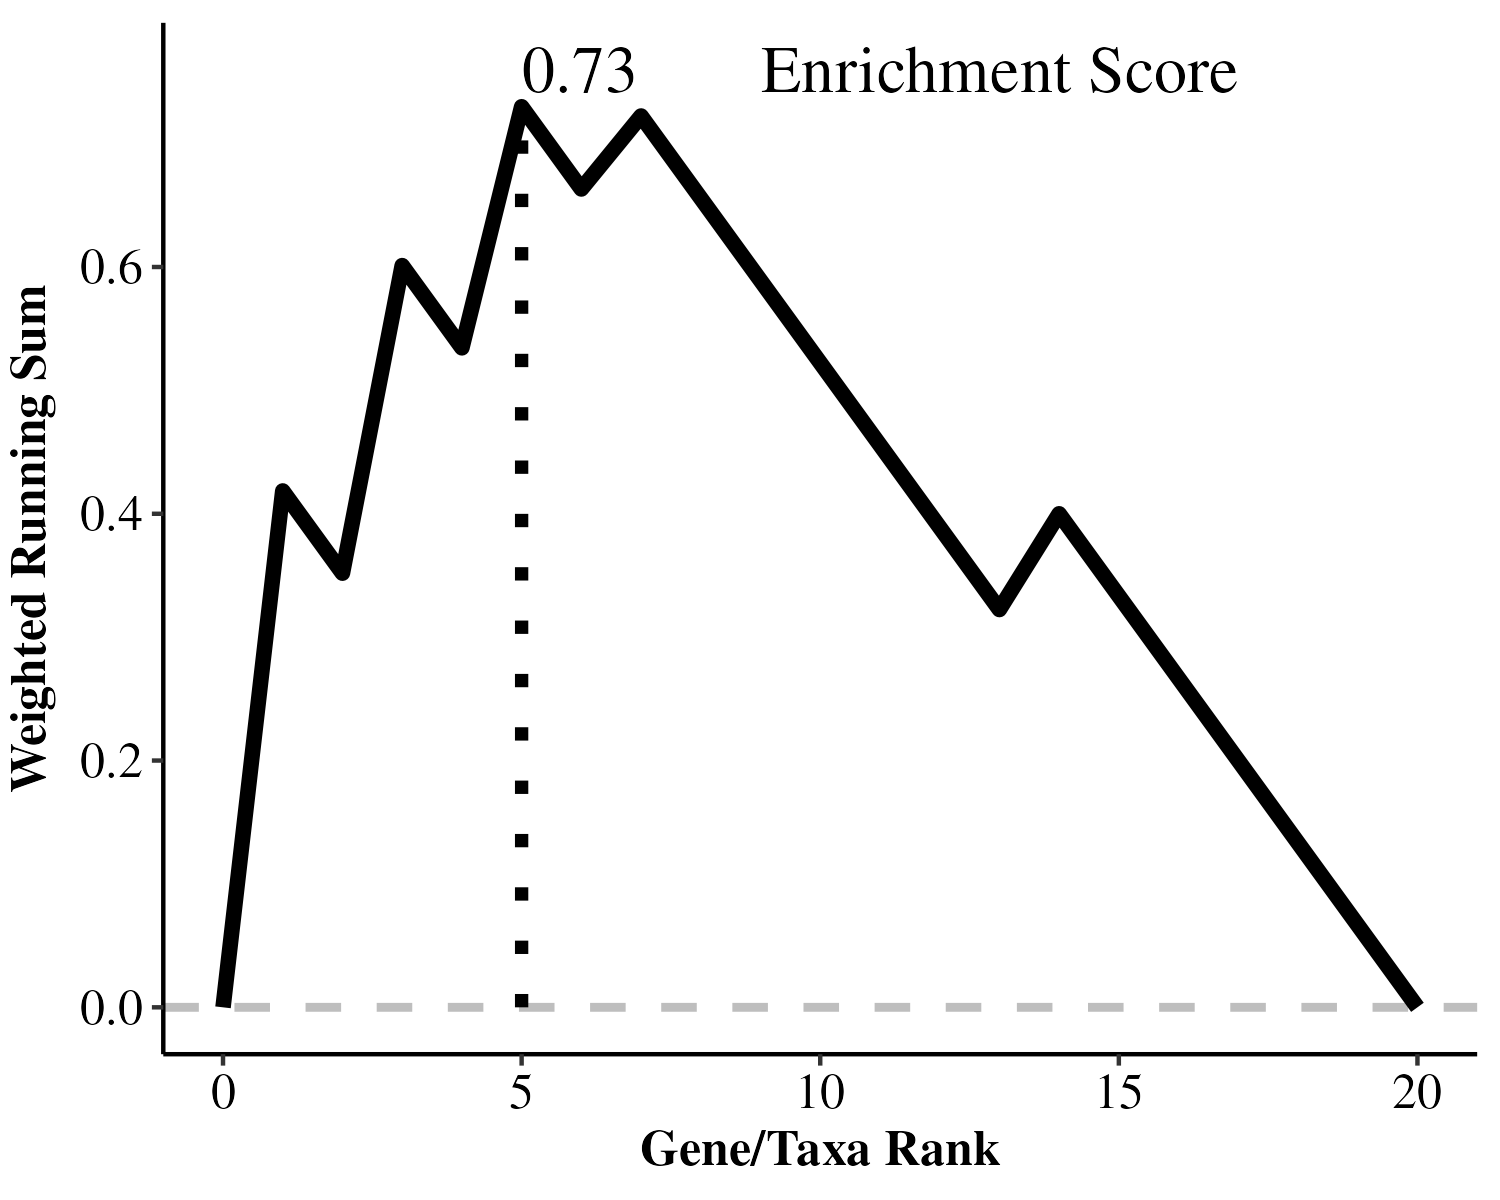
\includegraphics[scale=0.47]{/home/hh/data/output/lfcs_2.png}
        \end{center}
        \end{column}
    \end{columns}
  \end{enumerate} 
\end{frame}

\begin{frame}
   \frametitle{GSEA with Gene Label Permutations}

  The GSEA Algorithm Step-by-Step
  \begin{enumerate}
    \setcounter{enumi}{4}
    \item Calculate a null distribution of Enrichment Scores (ESs)
      \begin{alignat}{2}
        S &= \{\pmb{\text{ASK1}}, \pmb{\text{CHOP}}, \pmb{\text{TRAF2}}\} &&\implies \text{ES} \nonumber \\
        S^*_1 &= \{\pmb{\text{ASK1}}, \pmb{\text{CHOP}}, \text{B2M}\} &&\implies \text{ES}^*_1 \nonumber \\
         S^*_2 &= \{\text{BRCA1}, \text{EGFR}, \text{XRCC4}\}  &&\implies \text{ES}^*_2 \nonumber
      \end{alignat}
    \pause
    \item Use null distribution to calculate a p-value
  \end{enumerate} 
\end{frame}

\begin{frame}
  \frametitle{DSA Target Estimand}
  
  The goal of DSA is to estimate a \textbf{target estimand} \(\phi_S\):
  \begin{align*}
    \phi_S = \begin{cases}
      1 & \text{Gene Set } S \text{ is significantly enriched} \\
      -1 & \text{Gene Set } S \text{ is significantly depleted} \\
      0 & \text{Gene Set } S \text{ is not significantly changing}.
    \end{cases}
  \end{align*}

  \vspace{10px}

  In GSEA the target estimand is a function of the \textbf{true} LFCs:
  \begin{align*}
    \phi_S = g(\theta)
  \end{align*}

\end{frame}

\begin{frame}
  \frametitle{LFC Sensitivity Analysis}

  In GSEA the target estimand is a function of the \textbf{true} LFCs:
  \begin{align*}
    \phi_S = g(\theta)
  \end{align*}

  \vspace{10px}

  But we don't know the true LFCs, we only have \textbf{estimates}:
  \begin{align*}
    \hat{\phi}_S &= g(\hat{\theta}) \\
                 &= g(\hat{\theta}^\parallel + \underbrace{\hat{\theta}^\perp}_{\substack{\text{Estimated LFC in Scale} \\ \text{(Normalization Assumption)}}}).
  \end{align*}
  
  \pause

  \vspace{10px}
  
  Our DSA estimate \(\hat{\phi}_S\) \textbf{depends on our scale estimate} \(\hat{\theta}^\perp\)!

  \pause
  
  \begin{block}{LFC Sensitivity Analysis}
    A sensitivity analysis of how error in \(\hat{\theta}^\perp\) affects \(\phi_S\)
  \end{block}
  
\end{frame}

\begin{frame}
  \frametitle{LFC Sensitivity Analysis}

  Error \(\epsilon^\perp\) in our estimate of the unmeasured scale \(\theta^\perp\):
  \begin{align*}
    \underbrace{\theta^\perp}_{\text{True LFC in Scale}} = \underbrace{\hat{\theta}^\perp}_{\text{Estimate}} + \underbrace{\epsilon^\perp}_{\text{Estimation Error}}
  \end{align*}

  \pause
  
    How does the \textbf{true} \(\phi_S\) change with error \(\epsilon^\perp\)?
    \begin{align*}
      \phi_s &= g(\hat{\theta}^\parallel+ \hat{\theta}^\perp + \epsilon^\perp) \\
           &= g(\hat{\theta}+\epsilon^\perp)
    \end{align*}
  
  \pause

  LFC Sensitivity Analysis Algorithm:
  \begin{enumerate}
    \item Get estimated LFCs \(\hat{\theta}\) (e.g., from ALDEx2, limma, DESeq2, etc.)
    \pause
    \item Run GSEA with \(\epsilon^\perp=0\) (i.e., \(\hat{\phi}_S=g(\hat{\theta})\))
    \pause
    \item Rerun GSEA with \(\epsilon^\perp \neq 0\) and compare to \(\epsilon^\perp=0\) (i.e., \(\phi_S=g(\hat{\theta}+\epsilon^\perp\))
  \end{enumerate}

\end{frame}

\begin{frame}
  \frametitle{Interpreting Error \(\epsilon^\perp\) and LFC Sensitivity Analysis Results}

  Consider error \(\epsilon^\perp = \pm 0.5\):
  \begin{enumerate}
  \item This error corresponds to the true \(\theta^\perp\) being \(e^{0.5}=1.65\) times lower/higher than \(\hat{\theta}^\perp\)
    \pause
    \item Example results if a Gene set \(S\) is sensitive to error:
      \begin{center}
        \begin{tabular}{ |c|c|c| } 
        \hline
        \(\epsilon^\perp=-0.5\) & \(\epsilon^\perp=0\) & \(\epsilon^\perp=0.5\) \\
        \hline
        \(\phi_S=0\) & \(\phi_S=1\) & \(\phi_S=0\) \\
        \hline
        \end{tabular}
      \end{center}
    \pause
    \item Example results if a Gene set \(S\) is not sensitive to error:
      \begin{center}
        \begin{tabular}{ |c|c|c| }
        \hline
        \(\epsilon^\perp=-0.5\) & \(\epsilon^\perp=0\) & \(\epsilon^\perp=0.5\) \\
        \hline
        \(\phi_S=1\) & \(\phi_S=1\) & \(\phi_S=1\) \\
        \hline
        \end{tabular}
      \end{center}
  \end{enumerate}
\end{frame}

\begin{frame}
  \frametitle{LFC Sensitivity Analysis Simulation}
  
  \begin{center}
    \includegraphics[scale=0.65]{/home/hh/data/output/journal.pcbi.1011659.g001.PNG}
  \end{center}

  \small{PPV (Positive Predictive Value) is the \% of positives that are true positives}
 
\end{frame}

\begin{frame}
  \frametitle{Multiple Simulations of Different LFC Distributions, Gene Set Sizes, and Total \#'s of Genes}
  \begin{center}
    \includegraphics[scale=0.185]{/home/hh/data/output/fig_mult_sim.png}
  \end{center}
\end{frame}
  
\begin{frame}
  \frametitle{Real Data Analysis}

  \underline{RNA-seq: normal-adjacent-to-tumor vs. healthy thyroid tissue*}
  \begin{enumerate}
    \item LFCs estimated with Songbird (Morton et al., 2019)
    \item GSEA performed with fgsea (Korotkevich et al., 2021)
  

  \pause

  \item fgsea results for the Inflammatory Response Pathway:
  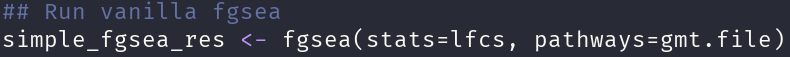
\includegraphics[scale=0.30]{/home/hh/data/output/vanilla_fgsea.png}
    \begin{center}
    \begin{tabular}{ |c|c| }
    \hline
    (Normalized) Enrichment Score & Adjusted p-value \\
    \hline
    \textcolor{blue}{1.53} & \textcolor{red}{0.003}  \\
    \hline
    \end{tabular}
    \end{center}
 
  \pause
  \item LFC Sensitvity Analysis results:
  \includegraphics[scale=0.30]{/home/hh/data/output/LFCS_fgsea.png}
    \begin{center}
    \begin{tabular}{ |c|c|c| }
    \hline
    \(\epsilon^\perp\) & (Normalized) Enrichment Score & Adjusted p-value \\
    \hline
    -0.5 & \textcolor{red}{-0.89} & 1  \\
    \hline
    0 & \textcolor{blue}{1.53} & \textcolor{red}{0.003}  \\
    \hline
    0.5 & \textcolor{blue}{1.5} & \textcolor{red}{0}  \\
    \hline
    \end{tabular}
    \end{center}
   \end{enumerate} 
\tiny{*(Aran et al., 2017)}
\end{frame}

\begin{frame}
  \frametitle{Complete Results for Real Data Analysis}
  
  \includegraphics[scale=0.75]{/home/hh/data/output/journal.pcbi.1011659.g002.PNG}
\end{frame}

\begin{frame}
  \frametitle{Two Additional Methods to Address False Positives}
  \pause
  \begin{enumerate}
  \item \underline{The LFC Sensitivity Test}

    \vspace{5px}
    Let \(p_{\epsilon^\perp}\) be the GSEA p-value at \(\epsilon^\perp\). Take the maximum GSEA p-value across all possible scale errors \(\epsilon^\perp \in (-\infty, \infty)\):
    \begin{align*}
      p=\sup_{\epsilon^\perp \in (-\infty, \infty)} p_{\epsilon^\perp}
    \end{align*}

    \begin{center}
      \includegraphics[scale=0.15]{/home/hh/data/output/power.png}
    \end{center}


  \end{enumerate}  
\end{frame}

\begin{frame}
  \frametitle{Two Additional Methods to Address False Positives}
  \begin{enumerate}
   \setcounter{enumi}{1}
   \item \underline{GSEA with Compositional Weighting (GSEA-CW)}

    \vspace{5px}
    The GSEA target estimand (i.e., goal of inference) is
    \begin{align*}
      \phi_S = g(\theta)
    \end{align*}

    \pause

    The GSEA-CW target estimand is different, and implies a different scientific question
    \begin{align*}
      \psi_S &= g(\theta^\parallel)
    \end{align*}

    \pause
    
  \end{enumerate}
\end{frame}
  
\begin{frame}
  \frametitle{DSA Methods that Account for Inter-gene/inter-taxa Correlations}
  Inter-gene/taxa correlations can massively inflate the false positive rate of GSEA with gene label permutations (Gatti et al., 2010)

  \begin{center}
    \includegraphics[scale=0.12]{/home/hh/data/output/correlations.png}
  \end{center}
  
  Two methods that handle inter-gene/taxa correlations:
  \begin{enumerate}
    \item GSEA with \textbf{sample label} permutations
    \item limma's CAMERA method
  \end{enumerate}
  
\end{frame}

\begin{frame}
  \frametitle{The CAMERA Method}
  

  Two methods that handle inter-gene/taxa correlations:
  \begin{enumerate}
  \item GSEA with \textbf{sample label} permutations
   \vspace{10px}
    
   Permute the sample labels (e.g., whether sample \(n\) came from healthy or tumor tissue), then re-estimate LFCs \(\hat{\theta}\)

   \pause
    
  \item limma's CAMERA method

    \vspace{10px}
    A two-sample t-test for the set \(S\) that uses a Variance Inflation Factor (VIF) to account for correlation:
    \begin{align*}
      \frac{\hat{\theta}_{\in S} - \hat{\theta}_{\notin S}}{s_p\sqrt{\text{VIF}/m_1+1/m_0}}
    \end{align*} 

  \end{enumerate}
\end{frame}

\begin{frame}
  \frametitle{Scale Sensitivity Analyses}
  \footnotesize{Here I consider two real data studies:}
  \begin{enumerate}
    \item \footnotesize{Constant Error \(\delta^\perp\) added to just samples from normal-adjacent-to-tumor}
    \item \footnotesize{Variable Error simulated from \(\text{Uniform}[-\gamma^\perp,\gamma^\perp]\) added to all samples}
  \end{enumerate}
   \begin{center}
    \includegraphics[scale=0.16]{/home/hh/data/output/camera.png}
   \end{center}

   \footnotesize{* GSEA-LFC-S is GSEA with sample label permutations, GSEA-CW-S is GSEA with compositional weighting and sample label permutations}
\end{frame}

\begin{frame}
  \frametitle{Future Directions}

  The LFC Sensitivity Test considers all possible errors \(\epsilon^\perp \in (-\infty, \infty)\):
  \begin{align*}
    p = \sup_{\epsilon^\perp \in (-\infty,\infty)} p_{\epsilon^\perp}
  \end{align*}

  \pause

  \vspace{10px}
  But why consider \textit{all} possible errors? For instance \(\theta^\perp=10\) might imply total transcription is 22,000 times higher in tumor than healthy tissue!

  \pause
  
  \vspace{10px}
  Rather assume \(\epsilon^\perp \in [-1,1]\):
  \begin{align*}
    p = \sup_{\epsilon^\perp \in [-1,1]} p_{\epsilon^\perp}
  \end{align*}

  \pause
  
\end{frame}

\begin{frame}
  \frametitle{Future Directions}

  In the previous presentation, SSRVs were a Bayesian approach to LFC estimation
  \begin{align*}
    \theta^\perp &= \hat{\theta}^\perp + \epsilon^\perp \\
    \epsilon^\perp &\sim P
  \end{align*}
  Where \(P\) is a user-defined distribution of scale uncertainty.

  \pause

  \vspace{10px}

  What if we take a \textit{purely Frequentist} approach? Rather than define \(P\) we just assume:
  \begin{align*}
    \theta^\perp \in [\hat{\theta}^\perp_L, \hat{\theta}^\perp_U]
  \end{align*}

  Let \(p_{\hat{\theta}^\perp}\) be the p-value under a single normalization assumption \(\hat{\theta}^\perp\), we can define a new p-value:
  \begin{align*}
    p = \sup_{\hat{\theta}^\perp \in [\hat{\theta}^\perp_L,\hat{\theta}^\perp_U]} p_{\hat{\theta}^\perp}
  \end{align*}
\end{frame}

\begin{frame}
  \frametitle{References}

  \begin{enumerate}   
  \item \footnotesize{Gatti, et al. Heading down the wrong pathway: on the influence of correlation within gene sets. BMC Genomics. 2010 Oct 18;11:574. doi: 10.1186/1471-2164-11-574.}
  \item \footnotesize{McGovern, et al. Addressing erroneous scale assumptions in microbe and gene set enrichment analysis. PLoS Comput Biol. 2023 Nov 20;19(11):e1011659. doi: 10.1371/journal.pcbi.1011659.}
   \item \footnotesize{Subramanian, et al. Gene set enrichment analysis: a knowledge-based approach for interpreting genome-wide expression profiles. Proc Natl Acad Sci U S A. 2005 Oct 25;102(43):15545-50. doi: 10.1073/pnas.0506580102. Epub 2005 Sep 30.}
   \item \footnotesize{Wu, et al. Camera: a competitive gene set test accounting for inter-gene correlation. Nucleic Acids Res. 2012 Sep 1;40(17):e133. doi: 10.1093/nar/gks461. Epub 2012 May 25.}
     \item \footnotesize{Aran, et al. Comprehensive analysis of normal adjacent to tumor transcriptomes. Nat Commun. 2017 Oct 20;8(1):1077. doi: 10.1038/s41467-017-01027-z. PMID: 29057876; PMCID: PMC5651823.}
  \end{enumerate}
  
\end{frame}

\end{document} 
